\documentclass{beamer}
\usetheme{Boadilla}
\usepackage{amsfonts,amsmath,amssymb}
\usepackage{braket,mathtools,siunitx}
\usepackage{hyperref}
\usepackage{textcomp,url}
\usepackage{graphicx}
\usepackage{listings,enumerate}
\usepackage{booktabs,tabularx,longtable,multicol}
\usepackage{subcaption}
\usepackage{float}

\lstset{language=C++}

\setbeamercovered{transparent}


\newcommand*\comment[2]{{\bf #1} \footnote{(#2)}}
\newcommand*\really[1]{\comment {#1} {really??? Need to verify this}}
\newcommand*\sayswho[1]{\comment {#1} {(who says this??? Need to find a citation)}}
\newcommand*\proveit[1]{\comment {#1} {(really? Can I show this??)}}

\newfloat{eqnfloat}{H}{eq}[section]
\floatname{eqnfloat}{Equation}

\newcommand*\limitset[1]{{#1}^\prime}
% Not working in unicode math with xelatex for some reason...
% \newcommand*\closure[1]{\overline #1}
\newcommand*\closureunion[1]{{#1}\cup \limitset{#1}}
\newcommand*\interior[1]{{#1}^\circ}

% Sets of points
% The set of points within some distance #1 from #2
\newcommand*\neighbor[2]{N_{#1}({#2})}
% The neighborhood without #2
\newcommand*\delneighbor[2]{N_{#1}^*({#2})}
% \newcommand*\set[1]{\{ #1 \} }
\newcommand*\conjugate[1]{\overline{#1}}
\newcommand*\sequence[2]{\set{#1}_{#2=1}^\infty}
\newcommand*\series[2]{\sum_{#2=1}^\infty #1_{#2}}
\newcommand*\compose[2]{#1 \circ #2}
\newcommand*\udisk{\mathbb{D}}
\newcommand*\disk[2]{D_{#1}(#2)}
\newcommand*\punctdisk[2]{\disk_{ #1 } - \set{#2}}
\newcommand*\complex{\mathbb{C}}
\newcommand*\naturals{\mathbb{N}}
\newcommand{\integers}{\mathbb{Z}}
\newcommand*\rationals{\mathbb{Q}}
\newcommand*\reals{\mathbb{R}}

\newcommand*\argmin{\text{argmin}}

% Function spaces
\newcommand*\cnfunc[2]{C^{#2}\left(#1 \right)}
\newcommand*\cnfuncdom[1]{C^{#1}\left(\domain \right)}
\newcommand*\linffunc[1]{L^{\infty}\left(#1 \right)}
\newcommand*\linffuncdom{L^{\infty}\left(\domain \right)}
\newcommand*\lnfunc[2]{L^{#2}\left(#1 \right)}
\newcommand*\lnfuncdom[1]{L^{#1}\left(\domain \right)}
\newcommand*\sobolev[3]{W^{#2, #3}\left(#1 \right)}
\newcommand*\sobolevdom[2]{W^{#1, #2}\left(\domain \right)}
\newcommand*\sobolevh[2]{H^{#2}\left(#1 \right)}
\newcommand*\sobolevhdom[1]{H^{#1}\left(\domain \right)}
\newcommand*\sobolevcs[3]{W_0^{#2, #3}\left(#1 \right)}
\newcommand*\sobolevcsdom[2]{W_0^{#1, #2}\left(\domain \right)}
\newcommand*\sobolevhcs[2]{H_0^{#2}\left(#1 \right)}
\newcommand*\sobolevhcsdom[1]{H_0^{#1}\left(\domain \right)}

\newcommand*\grad{D}
\newcommand*\graddir[1]{D_{#1}}
\newcommand*\lapl{∆}
\newcommand*\diffquot[1]{D^{#1}}
\newcommand*\diffquotdir[2]{D_{#2}^{#1}}

\newcommand*\domain{U}
\newcommand*\bndry[1]{\partial #1}
\newcommand*\bndrydom{\partial \domain}
\newcommand*\compactcont{\subset \subset} % U \compactcont V \rightarrow U \subset \closure{U} \subset V, where U, V are (open) domains

\newcommand*\ballunit{B_1}
\newcommand*\ball[2]{B_{#2}(#1)}
\newcommand*\bunitsurfarea[1]{\omega_{#1}}
\newcommand*\bunitsurfareadef{\omega_n}
\newcommand*\bunitvolume[1]{\alpha_{#1}}
\newcommand*\bunitvolumedef{\alpha_n}

\newcommand*\limitto[2]{\lim \limits_{#1 \rightarrow #2}}

\newcommand{\dd}[1]{\;\mathrm{d}#1}
\newcommand{\dx}{\dd{x}}
\newcommand{\dy}{\dd{y}}
\newcommand{\dz}{\dd{z}}
\newcommand{\dr}{\dd{r}}
\newcommand{\ds}{\dd{s}}
\newcommand{\dS}{\dd{S}}
\newcommand{\dt}{\dd{t}}
\newcommand*\pderiv[2]{\frac{\partial #1}{\partial #2}}
\newcommand*\nthpderiv[3]{\frac{\partial^{#3} #1}{\partial #2^{#3}}}
\newcommand*\deriv[2]{\frac{\dd{#1}}{\dd{#2}}}
\newcommand*\nthderiv[3]{\frac{\dd{^{#3} #1}}{\dd{#2^{#3}}}}

\newcommand*\abs[1]{\left| #1 \right|}

% Norms
\newcommand*\metricnorm[2]{\left\lVert#1\right\rVert_{#2}}

\newcommand*\linfnorm[2]{\left\lVert#1\right\rVert_{L^{\infty}(#2)}}
\newcommand*\linfnormdom[1]{\left\lVert#1\right\rVert_{L^{\infty}(\domain)}}

\newcommand*\lnorm[3]{\left\lVert#1\right\rVert_{L^{#2}(#3)}}
\newcommand*\lnormdom[2]{\left\lVert#1\right\rVert_{L^{#2}(\domain)}}
\newcommand*\frobnorm[1]{\left\lVert#1\right\rVert_{F}}

\newcommand*\hnorm[3]{\left\lVert#1\right\rVert_{H^{#2}(#3)}}
\newcommand*\hnormdom[2]{\left\lVert#1\right\rVert_{H^{#2}(\domain)}}

\newcommand*\wnorm[4]{\left\lVert#1\right\rVert_{W^{#2, #3}(#4)}}
\newcommand*\wnormdom[3]{\left\lVert#1\right\rVert_{W^{#2, #3}(\domain)}}

\newcommand*\vecnorm[1]{\left\lVert#1\right\rVert}

\DeclareMathOperator{\res}{res}
\DeclareMathOperator{\sign}{sign}
\DeclareMathOperator{\diam}{diam}
\DeclareMathOperator{\partition}{Partition}

% Matrix computations
\newcommand*\point[1]{{\bf{#1}}}
\renewcommand*\vector[1]{{\vec{\bf{#1}}}}
\newcommand*\trace[1]{\text{tr}\left( #1 \right)}
\newcommand*\transpose[1]{{#1}^{\intercal}}
\newcommand*\gradient[1]{\vector{\nabla} #1}
\newcommand*\divergence[1]{\vector{\nabla} \cdot #1}
\newcommand*\curl[1]{\vector{\nabla} \times #1}

% Common symbols
\newcommand*\metrictensor[0]{\mathcal{M}}
\newcommand*\elemenergy[1]{U_{#1}}
\newcommand*\elemmap[0]{\vector{M}}

% Average integral from https://tex.stackexchange.com/questions/759/average-integral-symbol
\def\Xint#1{\mathchoice
{\XXint\displaystyle\textstyle{#1}}%
{\XXint\textstyle\scriptstyle{#1}}%
{\XXint\scriptstyle\scriptscriptstyle{#1}}%
{\XXint\scriptscriptstyle\scriptscriptstyle{#1}}%
\!\int}
\def\XXint#1#2#3{{\setbox0=\hbox{$#1{#2#3}{\int}$ }
\vcenter{\hbox{$#2#3$ }}\kern-.6\wd0}}
\def\ddashint{\Xint=}
\def\dashint{\Xint-}
\def\avgint{\dashint}


\title{Adaptive Predicates Code Exploration}
\author{Michael Deakin}
\date{\today}

\begin{document}

\begin{frame}
  \titlepage
\end{frame}

\begin{frame}[fragile]
  \frametitle{Adaptive Polynomial Predicates}
  \begin{itemize}
  \item Detailed in Shewchuk's 1996 {\bf Adaptive Precision Floating-Point Arithmetic and Fast Robust Geometric Predicates}
  \item Some algorithms require correct (or at least consistent) floating point results, exact computations are slow
  \item Hand written only for specific computations, doesn't support vectorization, but very fast
  \end{itemize}
  My code is at \href{https://github.com/mfdeakin/adaptive_predicates}{github.com/mfdeakin/adaptive\_predicates}\\
  Overview:
  \begin{itemize}
  \item Introductory Test
  \item Expression Template Implementation
  \item Expression Template Evaluation
  \item Exact Evaluation Implementation
  \item Performance
  \item Adaptive Evaluation
  \item Performance
  \end{itemize}
\end{frame}

\begin{frame}[fragile]
  \frametitle{Adaptive Polynomial Predicates Test}
  {\href{https://github.com/mfdeakin/adaptive_predicates/blob/main/tests/test_adaptive_expr.cpp#L25}{github.com/mfdeakin/adaptive\_predicates/.../test\_adaptive\_expr.cpp\#L25}}
  \begin{lstlisting}[basicstyle=\small\ttfamily]
TEST_CASE("expr_template_structure",
	  "[expr_template]") {
  auto e = (arith_expr{} + 4.5 - 7) * 5;
  using E = decltype(e);
  static_assert(std::is_same_v<std::multiplies<>,
		               E::Op>);
  static_assert(std::is_same_v<std::minus<>,
		               E::LHS::Op>);
  static_assert(std::is_same_v<std::plus<>,
		               E::LHS::LHS::Op>);
  REQUIRE(e.rhs() == 5);
  REQUIRE(e.lhs().rhs() == 7);
  REQUIRE(e.lhs().lhs().rhs() == 4.5);

  REQUIRE(fp_eval<real>(e) == -12.5);
}
\end{lstlisting}

\end{frame}

\begin{frame}[fragile]
  \frametitle{arith\_expr implementation}
  \begin{lstlisting}[basicstyle=\small\ttfamily]
template <typename Op_, typename LHS_, typename RHS_>
class arith_expr final {
public:
  using LHS = std::remove_cvref_t<LHS_>;
  using RHS = std::remove_cvref_t<RHS_>;
  using Op = std::remove_cvref_t<Op_>;

  constexpr arith_expr(const LHS &lhs, const RHS &rhs)
      : m_lhs(lhs), m_rhs(rhs) {}
  constexpr arith_expr(LHS &&lhs, RHS &&rhs)
      : m_lhs(std::move(lhs)), m_rhs(std::move(rhs)) {}

  constexpr auto &lhs() const noexcept { return m_lhs; }
  constexpr auto &rhs() const noexcept { return m_rhs; }
  constexpr auto &operator()() { return *this; }
private:
  [[no_unique_address]] LHS m_lhs;
  [[no_unique_address]] RHS m_rhs;
};
\end{lstlisting}

\end{frame}

\begin{frame}[fragile]
  \frametitle{arith\_expr implementation}
  \begin{lstlisting}[basicstyle=\small\ttfamily]
template <class Op, class LHS_, class RHS_>
  requires arith_expr_operands<LHS_, RHS_> ||
           (arith_number<LHS_> && /* RHS... */)
auto make_expr(LHS_ &&lhs, RHS_ &&rhs) {
  using LHS = std::remove_cvref_t<LHS_>;
  using RHS = std::remove_cvref_t<RHS_>;
  return arith_expr<Op, LHS, RHS>(
    std::forward<LHS_>(lhs),
    std::forward<RHS_>(rhs));
}
template <typename LHS, typename RHS>
auto plus_expr(LHS &&lhs, RHS &&rhs) {
  return make_expr<std::plus<>>(
    std::forward<LHS>(lhs),
    std::forward<RHS>(rhs));
}
\end{lstlisting}

\end{frame}

\begin{frame}[fragile]
  \frametitle{arith\_expr evaluation}
  \begin{lstlisting}[basicstyle=\small\ttfamily]
template <std::floating_point eval_type,
          typename E_>
  requires expr_type<E_> || arith_number<E_>
constexpr eval_type fp_eval(E_ &&e) noexcept {
  using E = std::remove_cvref_t<E_>;
  if constexpr (is_expr_v<E>) {
    using Op = typename E::Op;
    return Op()(fp_eval<eval_type>(e.lhs()),
                fp_eval<eval_type>(e.rhs()));
  } else {
    return static_cast<eval_type>(e);
  }
}
\end{lstlisting}

\end{frame}

\begin{frame}[fragile]
  \frametitle{arith\_expr ``exact'' evaluation}
  Requires a representation of an exact quantity, use a finite series: % aka expansion sum
  $$(a_0, a_1, \ldots, a_n) = a_0 + a_1 + \ldots + a_n$$
  Then given exact representations $A$ and $B$ of lengths $n + 1$ and $m + 1$, scalar $s$, we can exactly compute addition, subtraction, and multiplication:
  \begin{itemize}
    \item $A + B = (a_0, a_1, \ldots, a_n, b_0, b_1, \ldots, b_m)$
    \item $A - B = (a_0, a_1, \ldots, a_n, -b_0, -b_1, \ldots, -b_m)$
    \item $A * s = (\text{two\_prod}(a_0, s), \text{two\_prod}(a_1, s), \ldots, \text{two\_prod}(a_n, s))$
    \item $A * B = A * b_0 + A * b_1 + \ldots + A * b_m$
  \end{itemize}
  where $\text{two\_prod}(a, b) = (a * b, fma(a, b, -a * b)$

  Requires a method of converting the result to a good representative of the floating point type, this project uses $\text{merge\_sum}$.
\end{frame}

\begin{frame}[fragile]
  \frametitle{arith\_expr ``exact'' evaluation}
  \begin{lstlisting}[basicstyle=\small\ttfamily]
template <std::floating_point eval_type, typename E>
  requires expr_type<E> || arith_number<E>
constexpr eval_type exactfp_eval(E &&e) noexcept {
    auto partial_results = ...;
    std::span<eval_type, num_partials_for_exact<E>()>
      partial_span{partial_results};
    _impl::exactfp_eval_impl<eval_type>(
      std::forward<E>(e), partial_span);
    return _impl::merge_sum(partial_span);
  } else {
    return static_cast<eval_type>(e);
  }
}
\end{lstlisting}

\end{frame}

\begin{frame}[fragile]
  \frametitle{arith\_expr ``exact'' evaluation}
  \href{https://github.com/mfdeakin/adaptive_predicates/blob/1caf304d6c502e619bcabdf51ab8696d52cff232/src/ae_fp_eval_impl.hpp#L127}{mfdeakin/adaptive\_predicates/.../src/ae\_fp\_eval\_impl.hpp\#L127}
\begin{lstlisting}[basicstyle=\small\ttfamily]
constexpr void exactfp_eval_impl(E_ &&e,
                                span_t partial_results)
 noexcept {
  // ...
  if constexpr (is_expr_v<E>) {
    const auto store_left =
      partial_results.template first</* ... */>();
    exactfp_eval_impl<eval_type>(e.lhs(), store_left);
    const auto store_right =
      partial_results.template subspan</* ... */>();
    exactfp_eval_impl<eval_type>(e.rhs(), store_right);
    // ...
  } else /* there is a runtime result */ {
    partial[0] = eval_type{e};
  }
}

\end{lstlisting}

\end{frame}

\begin{frame}[fragile]
  \frametitle{sparse\_mult implementation}
  \href{https://github.com/mfdeakin/adaptive_predicates/blob/1caf304d6c502e619bcabdf51ab8696d52cff232/src/ae_fp_eval_impl.hpp#L281}{github.com/mfdeakin/adaptive\_predicates/.../src/ae\_fp\_eval\_impl.hpp\#L281}
\begin{lstlisting}[basicstyle=\small\ttfamily]
template <std::ranges::range span_l,
          std::ranges::range span_r,
          std::ranges::range span_m>
void sparse_mult(span_l storage_left,
                 span_r storage_right,
                 span_m storage_mult) {
  auto out_i = storage_mult.end() - 1;
  for (auto r : storage_right | std::views::reverse) {
    for (auto l : storage_left | std::views::reverse) {
      auto [upper, lower] = exact_mult(r, l);
      *out_i = upper;
      --out_i;
      *out_i = lower;
      --out_i;
    }
  }
}
\end{lstlisting}

\end{frame}

\begin{frame}[fragile]
  \frametitle{merge\_sum implementation}
  \href{https://github.com/mfdeakin/adaptive\_predicates/blob/main/src/ae_fp_eval_impl.hpp#L252}{mfdeakin/adaptive\_predicates/.../src/ae\_fp\_eval\_impl.hpp\#L252}
\begin{lstlisting}[basicstyle=\small\ttfamily]
auto merge_sum_quadratic(auto &&storage) {
  auto out = storage.begin();
  for (eval_type &inp : storage | std::views::filter(
    [](const eval_type v) {
      return v != eval_type{0};
    })) {
    eval_type v = inp;
    auto [new_out, result] =
      merge_sum_append(storage.begin(), out, v);
    /* *** */
    *new_out = result;
    out = new_out + 1;
  }
  return *(out - 1);
  /* *** */
}
\end{lstlisting}

\end{frame}

\begin{frame}[fragile]
  \frametitle{merge\_sum implementation}
  \href{https://github.com/mfdeakin/adaptive_predicates/blob/main/src/ae_fp_eval_impl.hpp#L237}{mfdeakin/adaptive\_predicates/.../src/ae\_fp\_eval\_impl.hpp\#L237}
\begin{lstlisting}[basicstyle=\small\ttfamily]
auto merge_sum_append(auto begin, auto end, auto v) {
  using eval_type = decltype(v);
  auto out = begin;
  for (auto &e : std::span{begin, end}) {
    const auto [result, error] = two_sum(v, e);
    e = eval_type{0.0};
    v = result;
    if (error) {
      *out = error;
      ++out;
    }
  }
  return std::pair{out, v};
}
\end{lstlisting}

\end{frame}

\begin{frame}[fragile]
  \frametitle{Testing and Performance}
  Compute the orientation of points represented with double precision:
  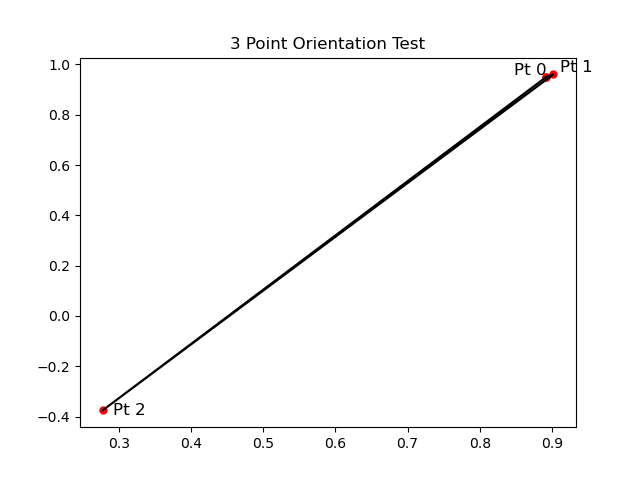
\includegraphics[width=0.475\linewidth]{images/orienttest.png}
  \hspace{1mm}
  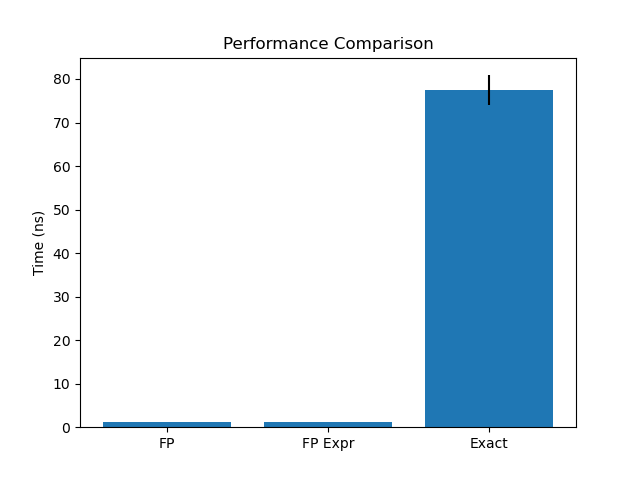
\includegraphics[width=0.475\linewidth]{images/exact_benchmark.png}\\
  
\includegraphics[width=20px]{images/scream.png} Exact evaluation takes $~63\times$ longer than floating point evaluation\\
  Use adaptive evaluation to avoid this cost
\end{frame}

\begin{frame}[fragile]
  \frametitle{Adaptive filter}
  Use a filter to detect when floats aren't enough.
  \href{https://github.com/mfdeakin/adaptive_predicates/blob/main/src/ae_fp_eval_impl.hpp#L107}{.../src/ae\_fp\_eval\_impl.hpp\#L107}
\begin{lstlisting}[basicstyle=\small\ttfamily]
template <typename Op>
std::pair<eval_type, eval_type> eval_with_max_abs_err(
  const eval_type left, const eval_type left_abs_err,
  const eval_type right, const eval_type right_abs_err) {
  if constexpr (/* is + or - */) {
    return {result, left_abs_err + right_abs_err +
                        std::abs(result) * epsilon / 2};

  } else if constexpr (/* is multiplies */) {
    return {result, right * left_abs_err +
                    left * right_abs_err +
                    left_abs_err * right_abs_err +
                    std::abs(result) * epsilon / 2};
  } else {
    return {result, NaN};
  }
}
\end{lstlisting}

\end{frame}

\begin{frame}[fragile]
  \frametitle{Adaptive evaluation}
  \href{https://github.com/mfdeakin/adaptive_predicates/blob/main/src/ae_adaptive_predicate_eval.hpp#L92}{.../src/ae\_adaptive\_predicate\_eval.hpp\#L92}
\begin{lstlisting}[basicstyle=\small\ttfamily]
template <typename sub_expr, typename branch>
std::pair<eval_type, eval_type>
adaptive_eval_impl::eval_impl(sub_expr &&expr) {
  auto &[result, memory = std::get<branch>(cache).get();
  if (result)
    return {*result, std::abs(*result) * epsilon / 2.0};

  auto [lr, le] =
    eval_impl<expr::LHS, /* left */>(expr.lhs());
  auto [rr, re] =
    eval_impl<expr::RHS, /* right */>(expr.rhs());
  const auto [result, max_abs_err] =
    eval_with_max_abs_err<Op>(lr, le, rr, re);
  if(max_abs_err > std::abs(result)) {
    /* Exact Eval Code... */
  } else return {result, max_abs_err};
}
\end{lstlisting}

\end{frame}

\begin{frame}[fragile]
  \frametitle{Adaptive performance}
  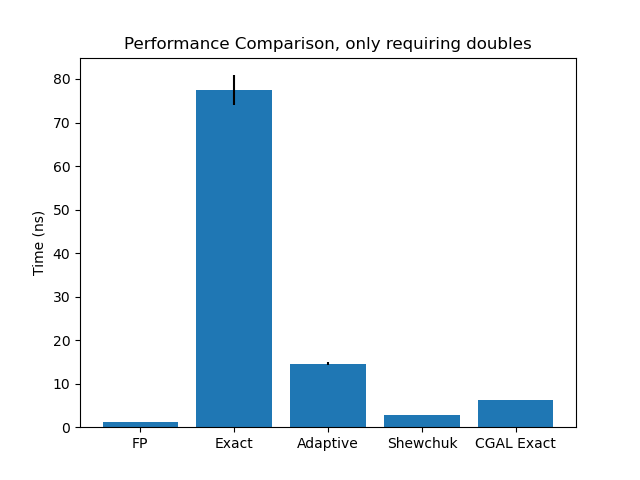
\includegraphics[width=0.475\linewidth]{images/adaptive_benchmark_fp.png}
  \hspace{1mm}
  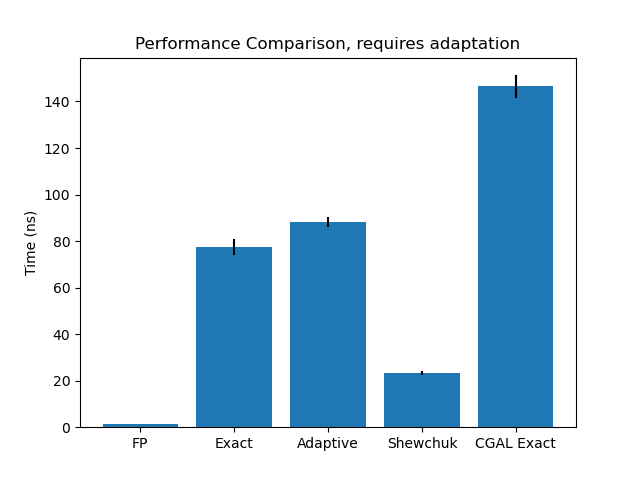
\includegraphics[width=0.475\linewidth]{images/adaptive_benchmark_exact.png}
\end{frame}

\begin{frame}
  \frametitle{Acknowledgements}
  \begin{centering}
    \hspace{5mm}
\includegraphics[width=1.0\linewidth]{images/collage.png}
  \end{centering}
\end{frame}

\end{document}
